\documentclass[border=4pt,12pt]{standalone}
% House style for redrawn exam diagrams (diagram-v4: 0.4pt lines, filled -latex arrows, fine dashes; stipple and hatching drawn as real dots/lines (no PDF/SVG patterns, so they render in every browser and at any scale); transparent background). Every figure \input's this.
\usepackage{amsmath,amssymb}
\usepackage{txfonts}
\usepackage{pdfrender,xcolor}
% \halo{text}: label on shading. The shading stops just around each letter's outline (a thin knock-out that follows the
% glyphs, like the papers' typesetting), never a box. Owner: "I don't want a box around the text".
\newcommand{\halo}[1]{\leavevmode\rlap{\pdfrender{TextRenderingMode=2,LineWidth=2.2pt,LineJoinStyle=1,StrokeColor=white,FillColor=white}#1}#1}
\usepackage{tikz,pgfplots}
\pgfplotsset{compat=1.18}
\usetikzlibrary{arrows.meta,calc,angles,quotes,patterns,patterns.meta,intersections,positioning,decorations.markings,shapes.geometric}
% Stipple and hatching are drawn as actual dots / lines clipped to the region (path picture), NOT as pattern fills:
% SVG <pattern> fills vanish or blur when browsers scale the image, so the owner could not see the shading.
% Each dot is a 0.72pt square (keeps SVGs small; reads as a dot at print size). Dots sit on one global staggered grid, so neighbouring regions line up.
\makeatletter
\newdimen\ex@x \newdimen\ex@y \newdimen\ex@xa \newdimen\ex@ya \newdimen\ex@xb \newdimen\ex@yb \newcount\ex@row
\def\exam@stipplecolor{black!75}\def\exam@dotr{0.42pt}\def\exam@dotgap{2.5}
\def\ex@rowdots{\ifdim\ex@x<\ex@xb \pgfpathrectangle{\pgfqpoint{\dimexpr\ex@x-0.36pt\relax}{\dimexpr\ex@y-0.36pt\relax}}{\pgfqpoint{0.72pt}{0.72pt}}\advance\ex@x by \exam@dotgap pt\relax\expandafter\ex@rowdots\fi}
\def\exam@stipple{%
  \pgftransformreset% dots are sized in real points even inside scaled pictures
  \pgfpointanchor{path picture bounding box}{south west}\ex@xa=\pgf@x \ex@ya=\pgf@y
  \pgfpointanchor{path picture bounding box}{north east}\ex@xb=\pgf@x \ex@yb=\pgf@y
  \pgfsetfillcolor{\exam@stipplecolor}\pgfmathsetmacro\ex@h{\exam@dotgap/2}%
  \pgfmathtruncatemacro\ex@r{floor(\ex@ya/\ex@h)-1}\ex@row=\ex@r\relax
  \ex@y=\ex@r\dimexpr\ex@h pt\relax
  \loop\ifdim\ex@y<\ex@yb
    \pgfmathtruncatemacro\ex@c{floor(\ex@xa/\exam@dotgap)-1}\ex@x=\ex@c\dimexpr\exam@dotgap pt\relax
    \ifodd\ex@row \advance\ex@x by \ex@h pt\fi
    \ex@rowdots
    \advance\ex@y by \ex@h pt \advance\ex@row by 1
    \ifnum\numexpr\ex@row-(\ex@row/4)*4\relax=0 \pgfusepath{fill}\fi% flush every 4 rows: bounded TeX memory, few clip copies in the SVG
  \repeat\pgfusepath{fill}}
\newdimen\ex@d
\def\exam@hatch#1{% #1 = 1 for /, -1 for \ ; lines 45 degrees, 3pt apart
  \pgftransformreset
  \pgfpointanchor{path picture bounding box}{south west}\ex@xa=\pgf@x \ex@ya=\pgf@y
  \pgfpointanchor{path picture bounding box}{north east}\ex@xb=\pgf@x \ex@yb=\pgf@y
  \ex@d=\dimexpr\ex@yb-\ex@ya\relax \ex@x=\dimexpr\ex@xa-\ex@d\relax
  \loop\ifdim\ex@x<\ex@xb
    \ifnum#1>0 \pgfpathmoveto{\pgfqpoint{\ex@x}{\ex@ya}}\pgfpathlineto{\pgfqpoint{\dimexpr\ex@x+\ex@d\relax}{\ex@yb}}%
    \else \pgfpathmoveto{\pgfqpoint{\ex@x}{\ex@yb}}\pgfpathlineto{\pgfqpoint{\dimexpr\ex@x+\ex@d\relax}{\ex@ya}}\fi
    \advance\ex@x by 4.24pt
  \repeat
  \pgfsetlinewidth{0.4pt}\pgfsetstrokecolor{black}\pgfusepath{stroke}}
\def\examstipple{\exam@stipple}\def\examhatch{\exam@hatch}\def\examsetstipplecolor#1{\def\exam@stipplecolor{#1}}\def\examsetdotgap#1{\def\exam@dotgap{#1}}
\makeatother
% (legacy pattern kept for old files)
% staggered stipple like the NESA papers' dotted shading
\pgfdeclarepatternformonly{exam stipple}{\pgfpointorigin}{\pgfqpoint{2.2pt}{2.2pt}}{\pgfqpoint{2.2pt}{2.2pt}}{%
  \pgfpathcircle{\pgfqpoint{0.55pt}{0.55pt}}{0.42pt}\pgfpathcircle{\pgfqpoint{1.65pt}{1.65pt}}{0.42pt}\pgfusepath{fill}}
\tikzset{
  every picture/.style={line width=0.6pt, >={Latex[length=2mm,width=1.3mm]}},
  curve/.style={line width=0.6pt},
  open arrow/.style={-{Latex[length=2mm,width=1.3mm]}},  % owner: filled -latex heads everywhere, no open chevrons
  aux/.style={dash pattern=on 2pt off 1.5pt, line width=0.6pt},
  shade/.code={\def\exA{#1}\def\exB{none}\ifx\exA\exB\else\pgfkeysalso{fill=black!18}\fi},
  shade/.default=on,
  shade dots/.style={fill=none, path picture={\examstipple}},
  stipple color/.code={\examsetstipplecolor{#1}},
  stipple gap/.code={\examsetdotgap{#1}},
  shade dense dots/.style={fill=none, stipple gap=1.6, path picture={\examstipple}},
  shade hatch/.style={fill=none, path picture={\examhatch{1}}},
  shade hatch reverse/.style={fill=none, path picture={\examhatch{-1}}},
  shade solid/.style={fill=black},
  pt/.style={circle, fill, inner sep=1.1pt},
  open pt/.style={circle, draw, fill=white, inner sep=1.1pt},
}
\pgfplotsset{
  exam axes/.style={axis lines=middle, axis line style={->}, xlabel={$x$}, ylabel={$y$},
    xlabel style={anchor=west}, ylabel style={anchor=south}, tick label style={font=\small},
    every axis plot/.append style={line width=0.6pt, black}, samples=200, clip=false,
    enlargelimits=false, axis on top},
}

\begin{document}
% crop pixel units (y down). Dots at the positions detected in the crop; frames, ticks and labels measured per panel.
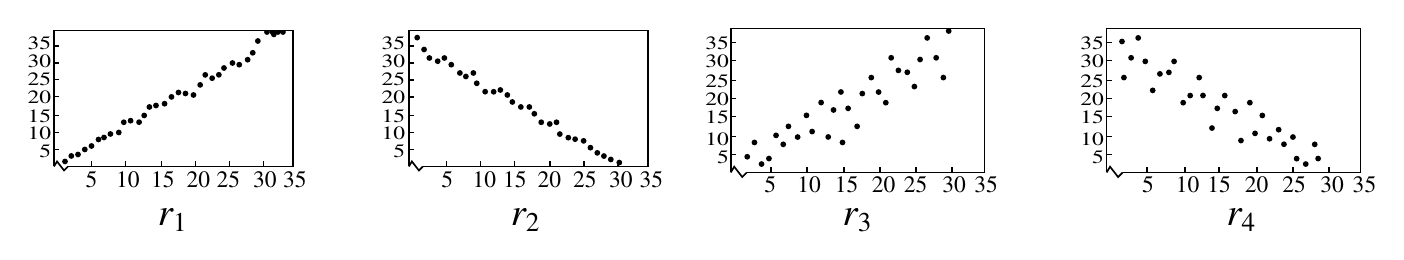
\begin{tikzpicture}[x=0.0127cm,y=-0.0127cm, every node/.style={inner sep=0pt}]
  % panel r1: 35 points
  \draw (27,153.5) -- (27,17.5) -- (266,17.5) -- (266,153.5) -- (41,153.5);
  \draw (27,153.5) -- (30,148.5) -- (37,157.5) -- (41,153.5);
  \foreach \t in {33,50,66.5,83.5,102.5,119.5,136.5} \draw (27,\t) -- (32,\t);
  \foreach \t in {64.5,98.5,134.5,168.5,202.5,236.5} \draw (\t,153.5) -- (\t,148.5);
  \begin{scope}\clip (27,17.5) rectangle (266,153.5);
    \foreach \p in {{(38.0,148.5)},{(44.3,143.0)},{(51.0,141.5)},{(57.8,136.5)},{(64.5,133.0)},{(71.5,126.5)},{(77.0,124.5)},{(83.4,121.0)},{(91.8,119.5)},{(96.8,109.3)},{(103.6,107.7)},{(112.1,109.2)},{(117.2,102.5)},{(122.4,94.0)},{(129.0,92.5)},{(137.6,90.7)},{(144.5,83.9)},{(151.5,79.5)},{(158.5,80.5)},{(166.5,82.0)},{(173.2,71.9)},{(178.3,61.9)},{(185.2,65.2)},{(191.9,61.8)},{(197.0,55.0)},{(205.5,50.0)},{(212.3,51.7)},{(220.7,46.7)},{(225.8,39.8)},{(230.9,28.0)},{(240.0,19.0)},{(245.5,19.0)},{(246.9,21.4)},{(251.0,19.0)},{(256.0,19.0)}} \fill \p circle[radius=2.9];
  \end{scope}
  \begin{scope}[every node/.append style={font=\fontsize{8.5}{9}\selectfont}]
    \node[anchor=east] at (25,30.5) {\scalebox{1}[0.8]{35}};
    \node[anchor=east] at (25,48) {\scalebox{1}[0.8]{30}};
    \node[anchor=east] at (25,66) {\scalebox{1}[0.8]{25}};
    \node[anchor=east] at (25,84.5) {\scalebox{1}[0.8]{20}};
    \node[anchor=east] at (25,103) {\scalebox{1}[0.8]{15}};
    \node[anchor=east] at (25,120.5) {\scalebox{1}[0.8]{10}};
    \node[anchor=east] at (25,138.5) {\scalebox{1}[0.8]{5}};
    \node[anchor=north] at (64.5,158) {5};
    \node[anchor=north] at (101,158) {10};
    \node[anchor=north] at (136,158) {15};
    \node[anchor=north] at (171.5,158) {20};
    \node[anchor=north] at (201.5,158) {25};
    \node[anchor=north] at (238,158) {30};
    \node[anchor=north] at (268,158) {35};
  \end{scope}
  \node[font=\fontsize{14}{16}\selectfont] at (146, 207) {$r_1$};
  % panel r2: 30 points
  \draw (382,153.5) -- (382,17.5) -- (621,17.5) -- (621,153.5) -- (396,153.5);
  \draw (382,153.5) -- (385,148.5) -- (392,157.5) -- (396,153.5);
  \foreach \t in {33,50,67,84,102.5,119.5,136.5} \draw (382,\t) -- (387,\t);
  \foreach \t in {419.5,453.5,487.5,523,557,591} \draw (\t,153.5) -- (\t,148.5);
  \begin{scope}\clip (382,17.5) rectangle (621,153.5);
    \foreach \p in {{(390.3,24.6)},{(397.2,36.5)},{(402.5,45.0)},{(410.8,48.2)},{(417.5,45.0)},{(424.4,51.7)},{(433.0,60.0)},{(439.0,63.5)},{(446.5,60.0)},{(449.9,70.3)},{(458.3,78.7)},{(466.8,78.8)},{(473.5,77.0)},{(480.5,82.0)},{(485.5,89.0)},{(494.0,94.0)},{(502.5,94.0)},{(507.5,100.8)},{(514.4,109.3)},{(522.9,111.0)},{(529.7,109.3)},{(533.0,121.1)},{(541.5,124.7)},{(548.3,126.2)},{(556.8,127.9)},{(563.6,134.7)},{(570.5,139.9)},{(577.1,143.1)},{(584.0,146.5)},{(592.5,149.6)}} \fill \p circle[radius=2.9];
  \end{scope}
  \begin{scope}[every node/.append style={font=\fontsize{8.5}{9}\selectfont}]
    \node[anchor=east] at (379,30.5) {\scalebox{1}[0.8]{35}};
    \node[anchor=east] at (379,48) {\scalebox{1}[0.8]{30}};
    \node[anchor=east] at (379,66) {\scalebox{1}[0.8]{25}};
    \node[anchor=east] at (379,84.5) {\scalebox{1}[0.8]{20}};
    \node[anchor=east] at (379,103) {\scalebox{1}[0.8]{15}};
    \node[anchor=east] at (379,120.5) {\scalebox{1}[0.8]{10}};
    \node[anchor=east] at (379,138.5) {\scalebox{1}[0.8]{5}};
    \node[anchor=north] at (420.5,158) {5};
    \node[anchor=north] at (457.5,158) {10};
    \node[anchor=north] at (488,158) {15};
    \node[anchor=north] at (522.5,158) {20};
    \node[anchor=north] at (558,158) {25};
    \node[anchor=north] at (594,158) {30};
    \node[anchor=north] at (624.5,158) {35};
  \end{scope}
  \node[font=\fontsize{14}{16}\selectfont] at (499, 207) {$r_2$};
  % panel r3: 30 points
  \draw (704,159.5) -- (704,15.5) -- (958,15.5) -- (958,159.5) -- (720.1,159.5);
  \draw (704,159.5) -- (707.45,153.75) -- (715.5,164.1) -- (720.1,159.5);
  \foreach \t in {29.5,47.5,67.5,85.5,103.5,123.5,141.5} \draw (704,\t) -- (709,\t);
  \foreach \t in {744,780,817.5,853.5,889.5,925.5} \draw (\t,159.5) -- (\t,154.5);
  \begin{scope}\clip (704,15.5) rectangle (958,159.5);
    \foreach \p in {{(720.5,143.8)},{(727.7,129.5)},{(734.8,151.1)},{(742.2,145.6)},{(749.3,122.4)},{(756.5,131.4)},{(761.7,113.4)},{(770.9,124.1)},{(779.7,102.4)},{(785.4,118.6)},{(794.4,89.6)},{(801.5,124.0)},{(806.8,97.0)},{(814.2,79.0)},{(815.8,129.5)},{(821.4,95.4)},{(830.4,113.4)},{(835.6,80.6)},{(844.6,64.6)},{(851.9,79.1)},{(859.1,89.7)},{(864.5,44.8)},{(871.7,57.4)},{(880.6,59.3)},{(887.7,73.6)},{(893.4,46.5)},{(900.5,24.9)},{(909.5,44.8)},{(916.7,64.6)},{(922.0,18.0)}} \fill \p circle[radius=2.9];
  \end{scope}
  \begin{scope}[every node/.append style={font=\fontsize{8.5}{9}\selectfont}]
    \node[anchor=east] at (703,30.5) {\scalebox{1}[0.8]{35}};
    \node[anchor=east] at (703,48.5) {\scalebox{1}[0.8]{30}};
    \node[anchor=east] at (703,68.5) {\scalebox{1}[0.8]{25}};
    \node[anchor=east] at (703,86.5) {\scalebox{1}[0.8]{20}};
    \node[anchor=east] at (703,104.5) {\scalebox{1}[0.8]{15}};
    \node[anchor=east] at (703,126) {\scalebox{1}[0.8]{10}};
    \node[anchor=east] at (703,144) {\scalebox{1}[0.8]{5}};
    \node[anchor=north] at (743.5,163) {5};
    \node[anchor=north] at (782.5,163) {10};
    \node[anchor=north] at (820,163) {15};
    \node[anchor=north] at (857,163) {20};
    \node[anchor=north] at (889,163) {25};
    \node[anchor=north] at (927.5,163) {30};
    \node[anchor=north] at (959.5,163) {35};
  \end{scope}
  \node[font=\fontsize{14}{16}\selectfont] at (831, 207) {$r_3$};
  % panel r4: 29 points
  \draw (1080,159.5) -- (1080,15.5) -- (1334,15.5) -- (1334,159.5) -- (1096.1,159.5);
  \draw (1080,159.5) -- (1083.45,153.75) -- (1091.5,164.1) -- (1096.1,159.5);
  \foreach \t in {29.5,47.5,67.5,85.5,103.5,123.5,141.5} \draw (1080,\t) -- (1085,\t);
  \foreach \t in {1120.5,1158.5,1192.5,1230.5,1266.5,1302.5} \draw (\t,159.5) -- (\t,154.5);
  \begin{scope}\clip (1080,15.5) rectangle (1334,159.5);
    \foreach \p in {{(1095.4,28.5)},{(1097.3,64.6)},{(1104.5,44.8)},{(1111.6,24.9)},{(1118.7,48.4)},{(1126.1,77.4)},{(1133.3,60.9)},{(1142.3,59.4)},{(1147.5,48.4)},{(1156.6,89.7)},{(1163.6,82.6)},{(1172.6,64.6)},{(1176.4,82.5)},{(1185.4,115.1)},{(1190.7,95.4)},{(1198.2,82.6)},{(1208.6,98.6)},{(1214.4,127.6)},{(1223.3,89.7)},{(1228.5,120.4)},{(1235.8,102.5)},{(1243.0,125.8)},{(1252.1,116.7)},{(1257.4,131.3)},{(1266.4,124.1)},{(1270.1,145.7)},{(1279.2,151.1)},{(1288.2,131.4)},{(1291.6,145.6)}} \fill \p circle[radius=2.9];
  \end{scope}
  \begin{scope}[every node/.append style={font=\fontsize{8.5}{9}\selectfont}]
    \node[anchor=east] at (1078,30.5) {\scalebox{1}[0.8]{35}};
    \node[anchor=east] at (1078,48.5) {\scalebox{1}[0.8]{30}};
    \node[anchor=east] at (1078,68.5) {\scalebox{1}[0.8]{25}};
    \node[anchor=east] at (1078,86.5) {\scalebox{1}[0.8]{20}};
    \node[anchor=east] at (1078,104.5) {\scalebox{1}[0.8]{15}};
    \node[anchor=east] at (1078,126) {\scalebox{1}[0.8]{10}};
    \node[anchor=east] at (1078,144) {\scalebox{1}[0.8]{5}};
    \node[anchor=north] at (1121.5,163) {5};
    \node[anchor=north] at (1161,163) {10};
    \node[anchor=north] at (1192.5,163) {15};
    \node[anchor=north] at (1230,163) {20};
    \node[anchor=north] at (1267.5,163) {25};
    \node[anchor=north] at (1305.5,163) {30};
    \node[anchor=north] at (1338,163) {35};
  \end{scope}
  \node[font=\fontsize{14}{16}\selectfont] at (1215, 207) {$r_4$};
\end{tikzpicture}
\end{document}